\documentclass[12pt, letterpaper]{article}

% ==========================================
%              DOCUMENT PACKAGES
% ==========================================

% --- Core Language & Encoding ---
\usepackage[english]{babel} % Sets the language and regional settings for English documents
\usepackage[utf8]{inputenc} % Allows the use of UTF-8 characters in the document
\usepackage[T1]{fontenc} % Specifies the font encoding
\usepackage[margin=2cm]{geometry} % Sets the page margins

% --- Colors & Graphics ---
\usepackage[table,dvipsnames]{xcolor} % Advanced color management
% \usepackage{color} % Basic package for text and background colors
\usepackage{graphicx} % Enhanced support for including external images and scaling them
\usepackage{adjustbox} % Adjusts the size, scaling, and alignment of boxes, images, and tables
% \usepackage{background} % Allows adding background images or watermarks to pages
\usepackage{float} % Improves the interface for floating objects and adds the [H] placement
\usepackage{pdflscape} % Makes landscape pages display correctly on screen in PDF viewers
\usepackage{pdfpages} % Allows the inclusion of external multi-page PDF documents

% --- Math, Science & Engineering ---
\usepackage{amsfonts} % Provides extended mathematical fonts
\usepackage{amsmath} % Provides advanced mathematical typesetting and environments
\usepackage{amssymb} % Provides extended mathematical symbols
% \usepackage{amsmath, amssymb} % (Redundant combination line omitted for stability)
\usepackage{amsthm} % Facilitates the creation of theorem-like environments
\usepackage{mathtools} % Enhances amsmath with additional math tools and bug fixes
\usepackage{thmtools} % Extensions and customization options for theorem environments
\usepackage{nicematrix} % Enhances matrices and tabulars using PGF/TikZ
\usepackage{xy} % Typesets complex graphs and diagrams
\usepackage{circuitikz} % Allows drawing of electrical networks and circuits

% --- Typography & Fonts ---
\usepackage{avant} % Sets the default sans-serif font to Avant Garde
\usepackage{cantarell} % Sets the default sans-serif font to Cantarell
\usepackage{charter} % Sets the default roman font to Charter
\usepackage{cmbright} % Sets the font family to Computer Modern Bright 
\usepackage{helvet} % Sets the default sans-serif font to Helvetica
\usepackage{inconsolata} % Sets the default typewriter (monospace) font to Inconsolata
\usepackage{iwona} % Sets the font family to Iwona 
\usepackage{kurier} % Sets the font family to Kurier 
\usepackage{lmodern} % Loads the Latin Modern fonts 
\usepackage{textcomp} % Provides additional text symbols
\usepackage{ulem} % Provides various types of text underlining and strikethroughs

% --- Tables & Lists ---
\usepackage{array} % Extends the array and tabular environments
\usepackage{arydshln} % Allows dashed lines in arrays and tables
\usepackage{bigstrut} % Adds custom vertical space in table rows
\usepackage{booktabs} % Enhances the quality of tables with better horizontal rules
% \usepackage{colortbl} % Allows coloring of rows, columns, and individual cells in tables
\usepackage{diagbox} % Creates table cells with diagonal lines
\usepackage{enumitem} % Provides advanced control over list environments
\usepackage{longtable} % Allows tables to break across multiple pages
\usepackage{multirow} % Allows individual table cells to span across multiple rows
\usepackage{tabularx} % Creates tables with dynamically adjustable-width columns
\usepackage{pgfplotstable} % Reads and cleanly formats numerical tables directly from CSV

% --- Formatting, Layout & UI ---
\usepackage{blindtext} % Generates dummy text for testing document layouts
\usepackage{caption} % Customizes captions in floating environments
\usepackage{comment} % Allows you to block out large sections of text
\usepackage{emptypage} % Automatically removes headers and footers on empty pages
\usepackage{fancyhdr} % Allows complete customization of headers and footers
\usepackage{fancyvrb} % Enhanced verbatim environments for writing raw code
\usepackage{framed} % Creates framed, shaded, or differently highlighted text regions
\usepackage{fullpage} % Quickly sets all page margins to 1 inch
\usepackage{lipsum} % Generates Lorem Ipsum dummy text
\usepackage{mdframed} % Creates highly customizable framed environments
\usepackage{multicol} % Allows intermixing single and multiple text columns
\usepackage{parskip} % Replaces standard paragraph indentation with vertical spacing
\usepackage{setspace} % Controls line spacing (single, one-and-a-half, double)
\usepackage{subcaption} % Supports sub-figures and sub-tables with independent captions
% \usepackage{subfig} % Older package for sub-figures (subcaption is generally preferred now)
\usepackage{tcolorbox} % Creates heavily customized colored and framed text boxes
\usepackage{titlesec} % Customizes the formatting of section, subsection, and chapter headings
\usepackage{titling} % Provides advanced control over the typesetting of the document title

% --- Bibliographies & References ---
\usepackage{biblatex} % Advanced, modern bibliographic processing and formatting
\usepackage{csquotes} % Context-sensitive quotation facilities
\usepackage{makeidx} % Supports the generation of a document index
% \usepackage{natbib} % Flexible bibliography support, particularly for author-year citation styles

% --- TikZ & Plotting ---
\usepackage{tikz} % Advanced package for creating vector graphics and diagrams programmatically
\usepackage{pgf-pie} % Draws pie charts programmatically using PGF/TikZ
\usepackage{pgfplots} % Creates high-quality mathematical plots, charts, and graphs
% \usepackage{fancytikzposter} % Used to create large format academic posters using TikZ

% --- URLs & Hyperlinks ---
\usepackage{url} % Formats and properly hyphenates long URLs
\usepackage{breakurl} % Allows line breaks in URLs, especially when compiled with latex -> dvips
\usepackage{hyperref} % Creates cross-referencing, clickable links, and PDF bookmarks

% --- Code Formatting ---
\usepackage{listings} % Typesets programming source code with formatting and syntax highlighting


% ==========================================
%           DOCUMENT CONFIGURATION
% ==========================================

% Custom color definitions
\definecolor{mygray}{gray}{0.9}

% Hyperlink configuration
\hypersetup{
    colorlinks=true,
    linkcolor=blue,
    urlcolor=blue
}

% Configuración adicional para breaks en URLs
\def\UrlBreaks{\do\/\do-\do_\do.\do=\do?\do\&}
\expandafter\def\expandafter\UrlBreaks\expandafter{\UrlBreaks\do\a\do\b\do\c\do\d\do\e\do\f\do\g\do\h\do\i\do\j\do\k\do\l\do\m\do\n\do\o\do\p\do\q\do\r\do\s\do\t\do\u\do\v\do\w\do\x\do\y\do\z}

%Uncomment the following lines to use a sans-serif font
%\renewcommand{\familydefault}{\sfdefault}

% TikZ libraries
\usetikzlibrary{shapes.geometric, positioning, decorations.pathreplacing}

\graphicspath{ {./img/} } % Sets the path for the graphics

\newlist{biblio}{enumerate}{1}
\setlist[biblio,1]{label=[\arabic*]}

\makeindex

% \tiny
% \scriptsize
% \footnotesize
% \small
% \normalsize (default size)
% \large
% \Large
% \LARGE
% \huge
% \Huge

% ==========================================
%         GLOBAL LISTINGS SETTINGS
% ==========================================
\lstset{
	basicstyle=\ttfamily\small,
	numbers=left,
	numberstyle=\tiny\color{gray},
	stepnumber=1,
	numbersep=10pt,
	backgroundcolor=\color{white},
	showspaces=false,
	showstringspaces=false,
	breaklines=true,
	frame=single,
	tabsize=2, 
    captionpos=b, 
    lineskip=-1pt,
	extendedchars=true,
	literate={á}{{\'a}}1 {é}{{\'e}}1 {í}{{\'i}}1 {ó}{{\'o}}1 {ú}{{\'u}}1 {Á}{{\'A}}1 {É}{{\'E}}1 {Í}{{\'I}}1 {Ó}{{\'O}}1 {Ú}{{\'U}}1 {ñ}{{\~n}}1 {Ñ}{{\~N}}1 {¿}{{\textquestiondown}}1 {¡}{{\textexclamdown}}1
}

% ==========================================
%            LANGUAGE: SQL
% ==========================================
\lstdefinestyle{sqlstyle}{
	language=SQL,
	keywordstyle=\color{blue}\bfseries,
	commentstyle=\color[rgb]{0,0.5,0}\itshape,
	stringstyle=\color{red}
}

% ==========================================
%            LANGUAGE: VHDL
% ==========================================
\lstdefinelanguage{VHDL}{
	morekeywords={entity, architecture, signal, port, in, out, inout, begin, end, process, if, then, else, elsif, case, when, others, for, while, loop, wait, library, use, std_logic, std_logic_vector, integer, boolean, rising_edge, falling_edge, component, generic, map, downto, to, and, or, not, xor, nand, nor, xnor},
	morecomment=[l]{--},
	morestring=[b]",
	sensitive=false,
	alsoletter={_}
}

\lstdefinestyle{vhdl}{
	language=VHDL,
	keywordstyle=\color{blue}\bfseries,
	commentstyle=\color[rgb]{0,0.6,0}\itshape,
	stringstyle=\color{red}
}

% ==========================================
%              LANGUAGE: C
% ==========================================
\lstdefinestyle{cstyle}{
	language=C,
	keywordstyle=\color{blue}\bfseries,
	commentstyle=\color[rgb]{0,0.5,0}\itshape,
	stringstyle=\color{red},
	directivestyle=\color{purple},
    tabsize=4 % Overrides the global tabsize of 2 for C code specifically
}

% ==========================================
%             LANGUAGE: C++
% ==========================================
\lstdefinestyle{cppstyle}{
	language=C++,
	keywordstyle=\color{blue}\bfseries,
	commentstyle=\color[rgb]{0,0.5,0}\itshape,
	stringstyle=\color{red},
	directivestyle=\color{purple},
    tabsize=4
}

% ==========================================
%           LANGUAGE: PYTHON
% ==========================================
\lstdefinestyle{pythonstyle}{
	language=Python,
	keywordstyle=\color{blue}\bfseries,
	commentstyle=\color[rgb]{0,0.5,0}\itshape,
	stringstyle=\color{red},
    % Python relies heavily on indentation, so keeping tabsize aligned is important
    tabsize=4
}

% ==========================================
%             LANGUAGE: BASH
% ==========================================
\lstdefinestyle{bashstyle}{
	language=bash,
	keywordstyle=\color{blue}\bfseries,
	commentstyle=\color[rgb]{0,0.5,0}\itshape,
	stringstyle=\color{red},
    % Bash variables often use $, so we can highlight them dynamically if needed
    moredelim=[s][\color{orange}]{\$\{}{\}}
}

% ==========================================
%           LANGUAGE: ASSEMBLY
% ==========================================
\lstdefinestyle{asmstyle}{
	language=[x86masm]Assembler,
	keywordstyle=\color{blue}\bfseries,
	commentstyle=\color[rgb]{0,0.5,0}\itshape,
	stringstyle=\color{red},
    % Adding common ARM/Microcontroller instructions for better highlighting
    morekeywords={ldr, str, mov, cmp, add, sub, b, bl, bx, push, pop, svc, eor, and, orr, lsl, lsr}
}

% % Configure header
\setlength{\headheight}{28pt} % Adjust header height for two-line header
\pagestyle{fancy}
\fancyhf{} % Clear all header and footer fields
\lhead{\textbf{Nombre:} Ugartechea González Luis Antonio -- 320223822 \\ \textbf{Asignatura:} <asignatura>, \textbf{Grupo:} <grupo>}
\renewcommand{\headrulewidth}{0.4pt}

\begin{document}

\begin{titlepage}

	\begin{tikzpicture}[remember picture,overlay]
		\node[anchor=north west, inner sep=30] at (current page.north west) {
			
\includegraphics[width=3.5cm, height=4cm]{escudoUNAM_color.png}
		};
		% \node[anchor=north west, inner sep=30] at (current page.north west) {
		% 	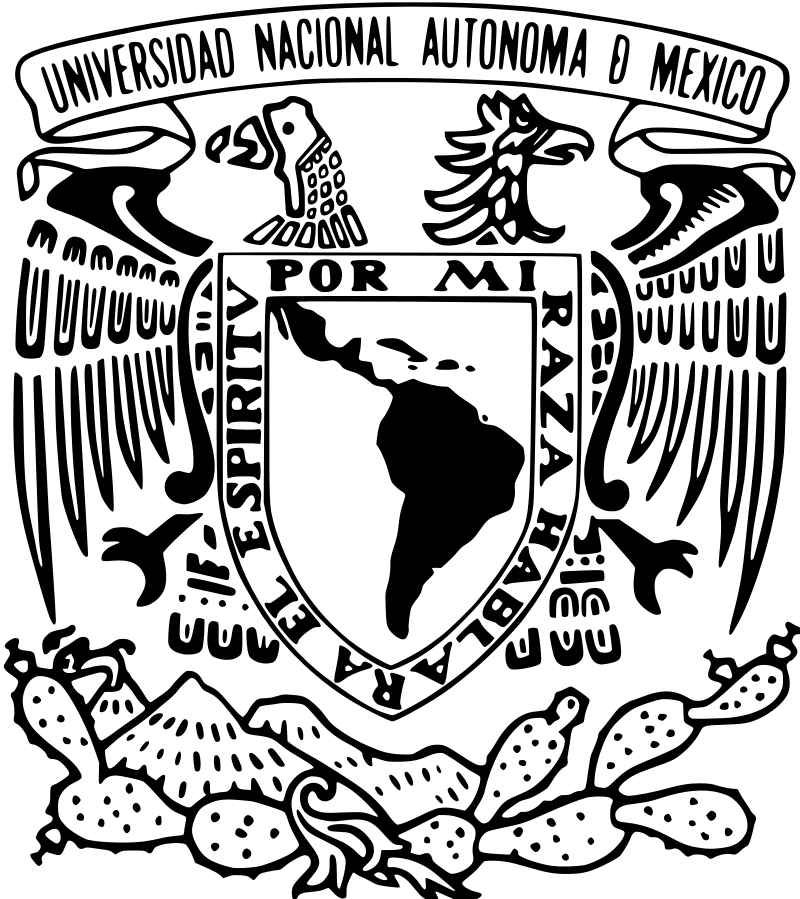
\includegraphics[width=4cm]{escudoUNAM_negro.png}
		% };

		\node[anchor=north east, inner sep=30] at (current page.north east) {
			
\includegraphics[width=3.5cm, height=4cm]{escudoFI_color.png}
		};
		% \node[anchor=north east, inner sep=30] at (current page.north east) {
		% 	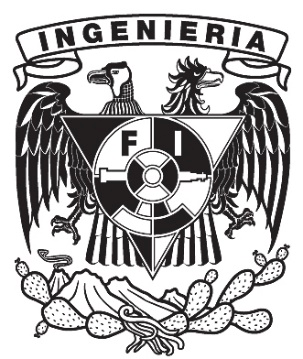
\includegraphics[width=4cm]{escudoFI_negro.png}
		% };
	\end{tikzpicture}

	\begin{center}
		\vspace*{1.5cm}

		\LARGE
		\textbf{Universidad Nacional Autónoma de México}\\
		Facultad de Ingeniería\\
		Ingeniería en Computación\\

		\Large
		\vspace*{1.5cm}
		\textbf{Sistemas Distribuidos}\\
		\vspace*{1.5cm}
		\large
		\textbf{Trabajo de Tecnologías y Tendencias Actuales en Sistemas Distribuidos}\\
	\end{center}

	\vspace*{1.5cm}
	\Large
	\textbf{Nombre de los Integrantes:}
	\begin{itemize}
		\item Ayala Hernández María Fernanda
		\item Saldaña Navarrete Andrea
		\item Tepal Briseño Hansel Yael
		\item Ugartechea González Luis Antonio
	\end{itemize}

	\vspace*{2cm}
	\textbf{Profesor(a):} M.I. Elba Karen Sáenz García \\
	\textbf{Grupo:} 3 \\
	\textbf{Semestre:} 2027-1 \\
	\textbf{Fecha de entrega:} 19 de noviembre de 2026 \\
\end{titlepage}

% Instrucciones
% Realizar una inves gación sobre el tema asignado que abarque los siguientes aspectos:
% 1. Concepto y funcionamiento: explicar qué es la tecnología seleccionada y cuáles son sus principios de funcionamiento.
% 2. Arquitectura: describir cómo está organizado el sistema, cuáles son sus componentes y qué función desempeña cada uno.
% 3. Comunicación y procesamiento: explicar cómo se comunican los componentes, cómo se distribuye el procesamiento y cómo se manejan los datos.
% 4. Problemas que resuelve: identificar qué necesidades o limitaciones de los sistemas tradicionales busca solucionar.
% 5. Aplicaciones reales: investigar una empresa, plataforma o proyecto que utilice esta tecnología.
% 6. Retos: identificar los principales desafíos técnicos y las posibles líneas de evolución.
% 7. Demostración práctica: incluir una pequeña demostración práctica o un ejemplo de funcionamiento. No es necesario desarrollar un sistema completo; pueden utilizar una simulación, un ejemplo de código, una herramienta existente o un diagrama que explique un escenario de funcionamiento.

\section{Introducción}

\section{Concepto y funcionamiento}

\section{Arquitectura}

\section{Comunicación y procesamiento}

\section{Problemas que resuelve}

\section{Aplicaciones reales}

\section{Retos}

\section{Demostración práctica}

\section{Conclusiones}

% \newpage
\section{Referencias}

\renewcommand{\refname}{}
\begin{biblio}
    \hypertarget{bonomi2012}{}
    \item Bonomi, F., Milito, R., Zhu, J., \& Addepalli, S. (2012). Fog computing and its role in the Internet of Things. En \textit{Proceedings of the First Edition of the MCC Workshop on Mobile Cloud Computing} (pp. 13--16). ACM. \url{https://doi.org/10.1145/2342509.2342513}
    \hypertarget{etsi2024}{}
    \item European Telecommunications Standards Institute. (2024). \textit{Multi-access Edge Computing (MEC); Framework and Reference Architecture} (ETSI GS MEC 003 V3.2.1). ETSI. \url{https://www.etsi.org/deliver/etsi_gs/MEC/001_099/003/03.02.01_60/gs_mec003v030201p.pdf}
    \hypertarget{ieee2018}{}
    \item IEEE Standards Association. (2018). \textit{IEEE Standard for Adoption of OpenFog Reference Architecture for Fog Computing} (IEEE Std 1934-2018). IEEE. \url{https://doi.org/10.1109/IEEESTD.2018.8423800}
    \hypertarget{iorga2018}{}
    \item Iorga, M., Feldman, L., Barton, R., Martin, M. J., Goren, N. S., \& Mahmoudi, C. (2018). \textit{Fog Computing Conceptual Model} (NIST Special Publication 500-325). National Institute of Standards and Technology. \url{https://doi.org/10.6028/NIST.SP.500-325}
    \hypertarget{meuser2024}{}
    \item Meuser, T., Lovén, L., Bhuyan, M., Patil, S. G., Dustdar, S., Aral, A., Bayhan, S., Becker, C., de Lara, E., Ding, A. Y., Edinger, J., Gross, J., Mohan, N., Pimentel, A. D., Rivière, E., Schulzrinne, H., Simoens, P., Solmaz, G., \& Welzl, M. (2024). Revisiting Edge AI: Opportunities and challenges. \textit{IEEE Internet Computing}, \textit{28}(4), 49--59. \url{https://doi.org/10.1109/MIC.2024.3383758}
    \hypertarget{openfog2017}{}
    \item OpenFog Consortium Architecture Working Group. (2017). \textit{OpenFog Reference Architecture for Fog Computing} (OPFRA001.020817). OpenFog Consortium. \url{https://www.digitaltwinconsortium.org/pdf/OpenFog_Reference_Architecture_2_09_17.pdf}
    \hypertarget{satyanarayanan2017}{}
    \item Satyanarayanan, M. (2017). The emergence of edge computing. \textit{Computer}, \textit{50}(1), 30--39. \url{https://doi.org/10.1109/MC.2017.9}
    \hypertarget{shi2016}{}
    \item Shi, W., Cao, J., Zhang, Q., Li, Y., \& Xu, L. (2016). Edge computing: Vision and challenges. \textit{IEEE Internet of Things Journal}, \textit{3}(5), 637--646. \url{https://doi.org/10.1109/JIOT.2016.2579198}
\end{biblio}

\end{document}
